\documentclass[12pt]{article}
\usepackage[utf8]{inputenc}

%%% I added a few packages. This next one allows you to set the margins.
\usepackage[top=.5in,bottom=1in,right=.75in,left=.75in]{geometry}
\usepackage{multicol}
%\usepackage{newspaper}
\setlength{\columnsep}{1cm}
\usepackage{blindtext}
\usepackage{varwidth}

%%% This one does boxes in a really nice way.
\usepackage{tcolorbox}
\usepackage{mdframed}
\usepackage{minibox}
\usepackage{graphicx}
\graphicspath{ {./images/} }
\usepackage{epstopdf}
  \epstopdfDeclareGraphicsRule{.pdf}{png}{.png}{convert #1 \OutputFile}
  \DeclareGraphicsExtensions{.png,.pdf}
\usepackage{hyperref}
\hypersetup{
    colorlinks=true,
    linkcolor=blue,
    filecolor=magenta,      
    urlcolor=cyan,
    pdftitle={MSCSMess},
    pdfpagemode=FullScreen,
    }
\urlstyle{same}
 \usepackage{fix-cm}
 \usepackage{soul}
 \usepackage{graphicx}
 \usepackage{multicol}


\newcommand{\ds}{\displaystyle}
\newcommand{\ZZ}{\mathbb{Z}}
\newcommand{\QQ}{\mathbb{Q}}
\newcommand{\RR}{\mathbb{R}}
\newcommand{\CC}{\mathbb{C}}
\newcommand{\FF}{\mathbb{F}}
\newcommand{\xx}{\mathbf{x}}
\newcommand{\uu}{\mathbf{u}}
\newcommand{\vv}{\mathbf{v}}

\newcommand{\bolder}{\textbf}
 
 
\title{\fontsize{60}{70}\selectfont {\bf {MSCS} 
\includegraphics[scale=.3]{images/OleLion.png} {Mess}}}
\author{Department of Mathematics, Statistics, and Computer Science \\ St.\@ Olaf College, Northfield, MN 55057 \vspace{-2ex}} 
\date{\today\, $|$ Volume 54, No.\@ 20 \line(1,0){500}}


\begin{document}

\maketitle \vspace{-1cm}
\begin{center}
We hope you all have a happy spring break! Hopefully you can take some time to rest and do something fun over the next week. See you in April :)
\end{center}

 \begin{multicols}{2}


 \begin{tcolorbox}[colback=white, colframe=black]
    \begin{center}
    \title{{\large \bolder{MSCS Gear is Back! (Final Sale of the Year)}}}
    \end{center}
\end{tcolorbox}

The MSCS department is excited to announce their final apparel sale of the year. If you have been waiting to grab some MSCS gear, now is the time to act. The deadline is Tuesday, April 7th at 11:59 PM, so be sure to place your order before the shop closes for the year. You can shop here: \href{larsonsprinting.itemorder.com/shop/}{Link to buy!} Use the access code SPRING26MSCS.


 \begin{tcolorbox}[colback=white, colframe=black]
    \begin{center}
    \title{{\large \bolder{Summer Math Job}}}
    \end{center}
\end{tcolorbox}
Are you looking for a summer job related to math? Would you enjoy working with kids? If so, consider applying to be a counselor at MathPath (\href{http://www.mathpath.org}{www.mathpath.org})!

MathPath is a residential summer camp for middle school students. This summer, the camp will be at the University of Portland (Oregon) from late June through most of July. 

MathPath is currently hiring counselors, who are typically college students enthusiastic about mathematics, who are very responsible, and who would enjoy working with children ages 11-14. For a detailed job description and application instructions, please see \href{https://www.mathpath.org/employment/counselors}{https://www.mathpath.org/employment}. You may disregard the February deadline -- applications are still being accepted! If you're interested, apply soon! 

If you have any questions about this job, talk with Prof. Wright (wright5@stolaf.edu) or email MathPath Camp Director April Verser (april.verser@mathpath.org).


 \begin{tcolorbox}[colback=white, colframe=black]
    \begin{center}
    \title{{\large \bolder{4/2 Carleton Talk: Human Factors, Computing, and Children}}}
    \end{center}
\end{tcolorbox}
The Department of Computer Science at Carleton College will be hosting Juan Pablo Hourcade speaking on “Human Factors, Computing, and Children” on Thursday, April 2 from 3:30 to 4:30 pm in Anderson 329. Professor Hourcade will be speaking on how to design technologies for interactions with children.  His visit is sponsored by the ACM Distinguished Speaker Program. Details about the event are available, and the event poster is attached below. Please reach out if you have any questions! 

\vfill\,

 \begin{tcolorbox}[colback=white, colframe=black]
    \begin{center}
    \title{{\large \bolder{Annual MSCS Talent Show!}}}
    \end{center}
\end{tcolorbox}
The MSCS Department is hosting the MSCS Recital on Wednesday, April 15th, at 7:00pm in Ytterboe Lounge!

The recital is an annual recognition of the talent (broadly defined), of the members of the MSCS community. Faculty and students will perform, in ensembles or solo, for an hour or two in the evening. Anyone associated with MSCS is welcome to participate, as a performer or an observer. This is a fun, relaxed gathering of students and faculty on equal footing. We sincerely hope you will join us!

There will be food and drink, including home cooking. If you are interested in performing or have questions, please contact Carlos Chávez (chavez16@stolaf.edu) or Daniel Stoertz (stoert1@stolaf.edu), or fill out \href{https://docs.google.com/forms/d/e/1FAIpQLSctO8sAXxTCjrrDK_F1ocOHFMjC1OTzejShYgvfoWYQjHmg1g/viewform?usp=publish-editor}{this interest form}.
 

\begin{tcolorbox}[colback=white, colframe=black]
    \begin{center}
    \title{{\large \bolder{Summer Opportunity in Math Education}}}
    \end{center}
\end{tcolorbox}

\href {https://bsmeducation.com} {Budapest Semesters in Mathematics Education (BSME)} is a 6-week summer program in Budapest, Hungary, designed for those interested in the learning and teaching of mathematics. Participants take a variety of courses in mathematics education and complete a week-long field experience. Come experience the \href{https://bsmeducation.com/wp-content/uploads/2020/02/hungarian-pedagogy-flyer.pdf}{Hungarian pedagogy} based on guided discovery—which emphasizes problem solving, mathematical creativity, and communication—as well as the rich and vibrant culture of Hungary.

Scholarships are available from the St. Olaf Financial Aid Office. See the \href{https://wp.stolaf.edu/smithcenter/st-olaf-summer-programs/#:~:text=All%20students%20are%20automatically%20considered%20for%20a%20need%2Dbased%20scholarship%20(see%20J%2DTerm%20column)%20of%20up%20to%2050%25%20of%20program%20costs%20from%20the%20St.%20Olaf%20Financial%20Aid%20Office.%C2%A0%C2%A0}{Smith Center's} webpage for more details. If you have any questions, contact Prof. Ryota Matsuura (matsuura@stolaf.edu).

\begin{tcolorbox}[colback=white, colframe=black]
    \begin{center}
    \title{{\large \bolder{Summer Offering - Math 226: Multivariable Calculus}}}
    \end{center}
\end{tcolorbox}
Looking for something productive and fun to do for the first part of the summer?  Come take an awesome math course!  Professor Salois will be offering a section of Math 226 for Summer Session I, which will meet 10:00-11:30 AM Tuesdays-Fridays.  Registration on SIS opened on Monday, March 2.  If you have any questions, please contact Prof. Kyle Salois (salois1@stolaf.edu). 



\begin{tcolorbox}[colback=white, colframe=black]
    \begin{center}
    \title{{\large \bolder{Problem Solving Group}}}
    \end{center}
\end{tcolorbox}
The Math Problem Solving Group meets weekly to have fun, solve math problems, eat candy, and prepare for upcoming math contests. Meetings are Thursdays from 11:30 am - 12:30 pm, in RNS 207 (the Center for Interdisciplinary Research room). Everyone is welcome, regardless of prior experience in mathematics or math contests!


\end{multicols} \vfill 

\begin{center}
    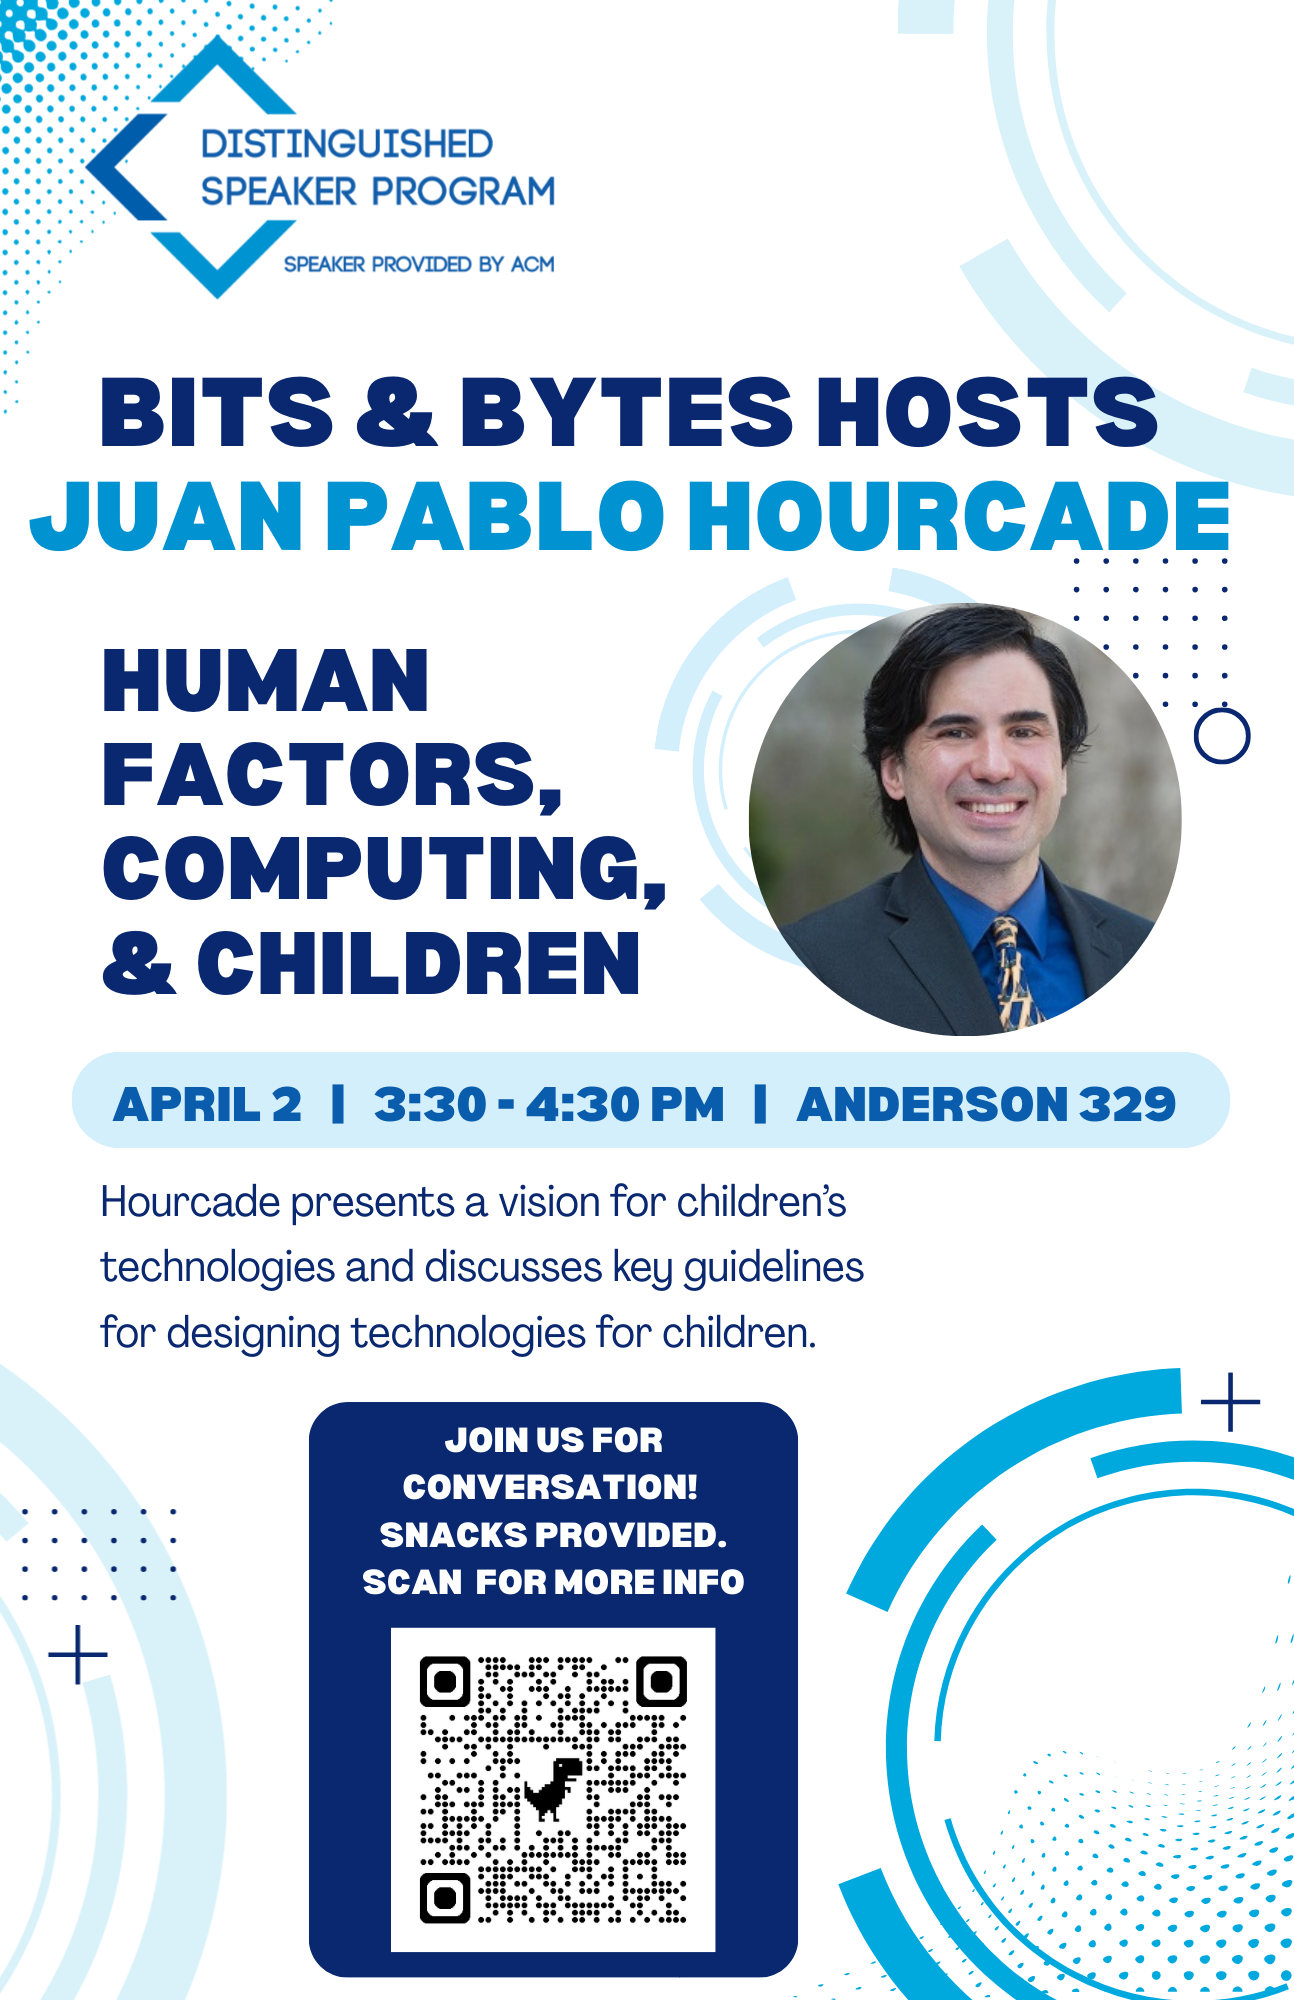
\includegraphics[height=0.95\textheight]{images/Bits & Bytes hosts JP Hourcade - 04022026.png}
\end{center}

\begin{center}
    
\includegraphics[height=0.95\textheight]{Apparel Sale (3).png}
\end{center}

\begin{center}
    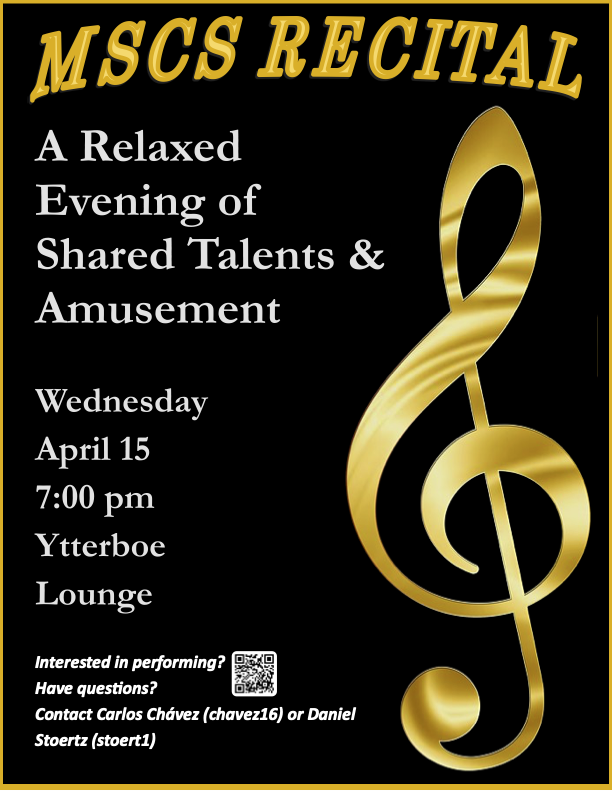
\includegraphics[height=0.95\textheight]{Recital Invite 26_qr.png}
\end{center}

\begin{center}
    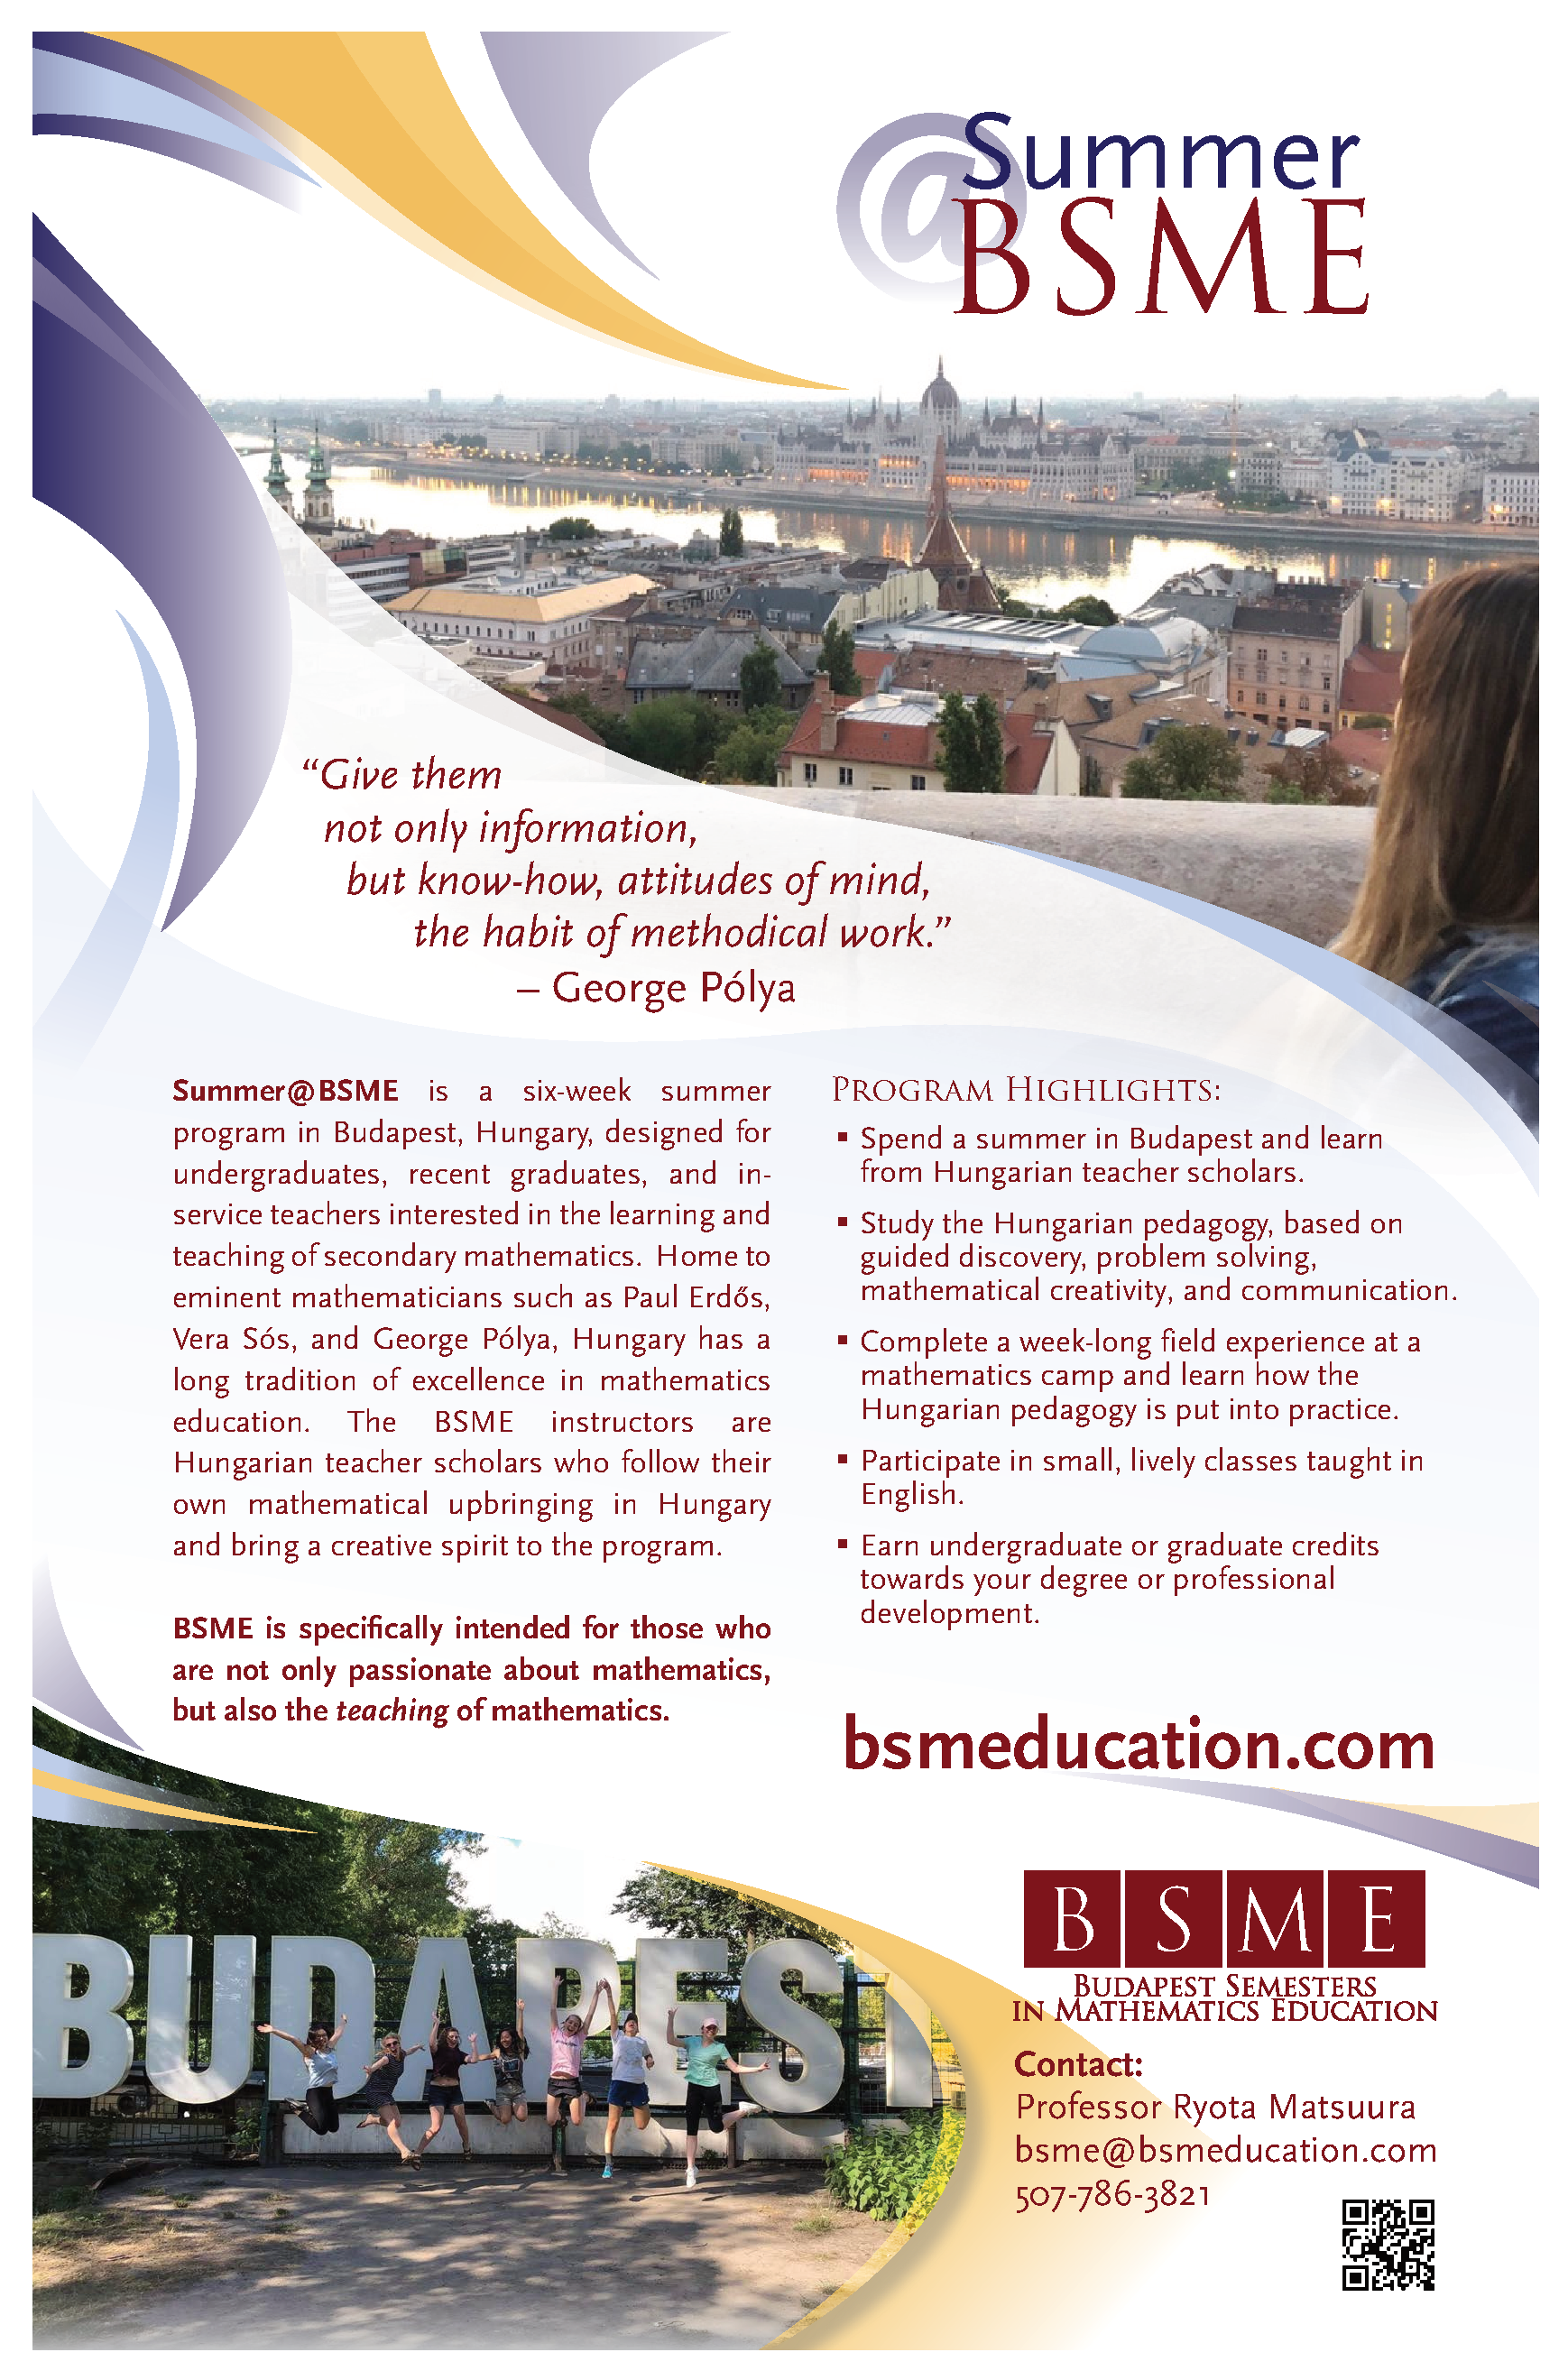
\includegraphics[height=0.95\textheight]{images/2024-bsme-poster-revised-web.pdf}
\end{center}

\begin{center}
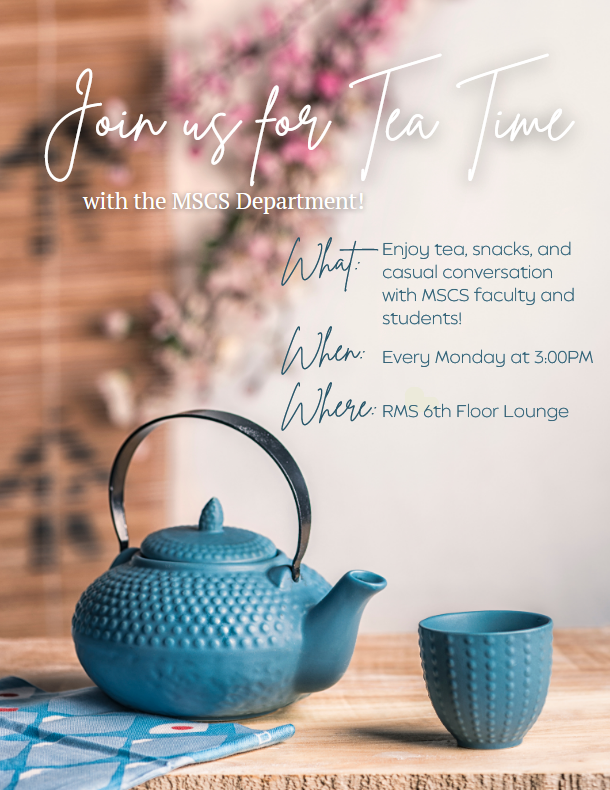
\includegraphics[width=0.9\textwidth]{images/Tea Time Poster.png}
\end{center}

\noindent{To submit an article, event, or anything else for publication in the Mess, email messeditor@stolaf.edu. Visit \href{https://wp.stolaf.edu/mscs/mscs-mess/}{http://wp.stolaf.edu/mscs/mscs-mess/} for a digital archive of previous MSCS Mess issues.}\\
	
\hfill Nima Dahir, Editor
	
\hfill Kyle Salois, Faculty Advisor


 

\end{document}